% fig1_methods -- conceptual architecture. Referee round 2 (2026-09-30): three stages and
% the novelty contrast. Feedback round 3 (2026-09-30 evening): fewer words per box, the
% source-level against vertex-level contrast enlarged into a full-width lower panel, and the
% two triple builders made visible (time-based in the acquisition column; the analysis column
% runs on triples grouped by simulated event identity). Method parameters live in the caption.
% Drawn at its printed width (about 150 mm); smallest text 8 pt. House palette (ejmp_style).
% Review round 6 (2026-10-08): the lower panel, the architecture difference the paper tests, is
% emphasized (panel letter d, heading, tinted frame); the upper chain is standard.
% Review round 16 (2026-10-19): four columns, the time-based clinical branch (c) beside the event-identity
% branch (d), so that the event builder, randoms arm and estimator are visible; the lower panel becomes (e).
\documentclass[tikz,border=2pt]{standalone}
\IfFileExists{stix.sty}{\usepackage{stix}}{\IfFileExists{mathptmx.sty}{\usepackage{mathptmx}}{}}
\usetikzlibrary{positioning,arrows.meta,calc,fit,backgrounds,decorations.pathmorphing}

\definecolor{hblue}{HTML}{3D5A80}
\definecolor{hgreen}{HTML}{0F7173}
\definecolor{hgrey}{HTML}{8A8988}

\newcommand{\sev}{\fontsize{8}{9.2}\selectfont}
\tikzset{
  every node/.style={font=\fontsize{8.2}{9.4}\selectfont},
  box/.style={draw, line width=0.5pt, rounded corners=1.2pt, align=center,
              text width=33mm, inner xsep=2pt, inner ysep=2.4pt, minimum height=7.4mm},
  phy/.style={box, draw=hblue, fill=hblue!10},
  acq/.style={box, draw=black!55, fill=black!4},
  ana/.style={box, draw=hgreen, fill=hgreen!9},
  key/.style={phy, fill=hblue!26, line width=1.0pt},
  tag/.style={draw=black!60, dashed, line width=0.5pt, rounded corners=1.2pt, fill=white, align=center,
              font=\sev, inner xsep=2pt, inner ysep=1.6pt, text width=33mm},
  arr/.style={-{Stealth[length=1.7mm, width=1.3mm]}, line width=0.55pt, draw=black!70, rounded corners=1pt},
  head/.style={font=\fontsize{9}{10}\selectfont\bfseries, anchor=south},
  sub/.style={font=\sev, text=black!62},
}
\newcommand{\sd}[1]{\\[-1pt]{\sev\color{black!62}#1}}

\begin{document}
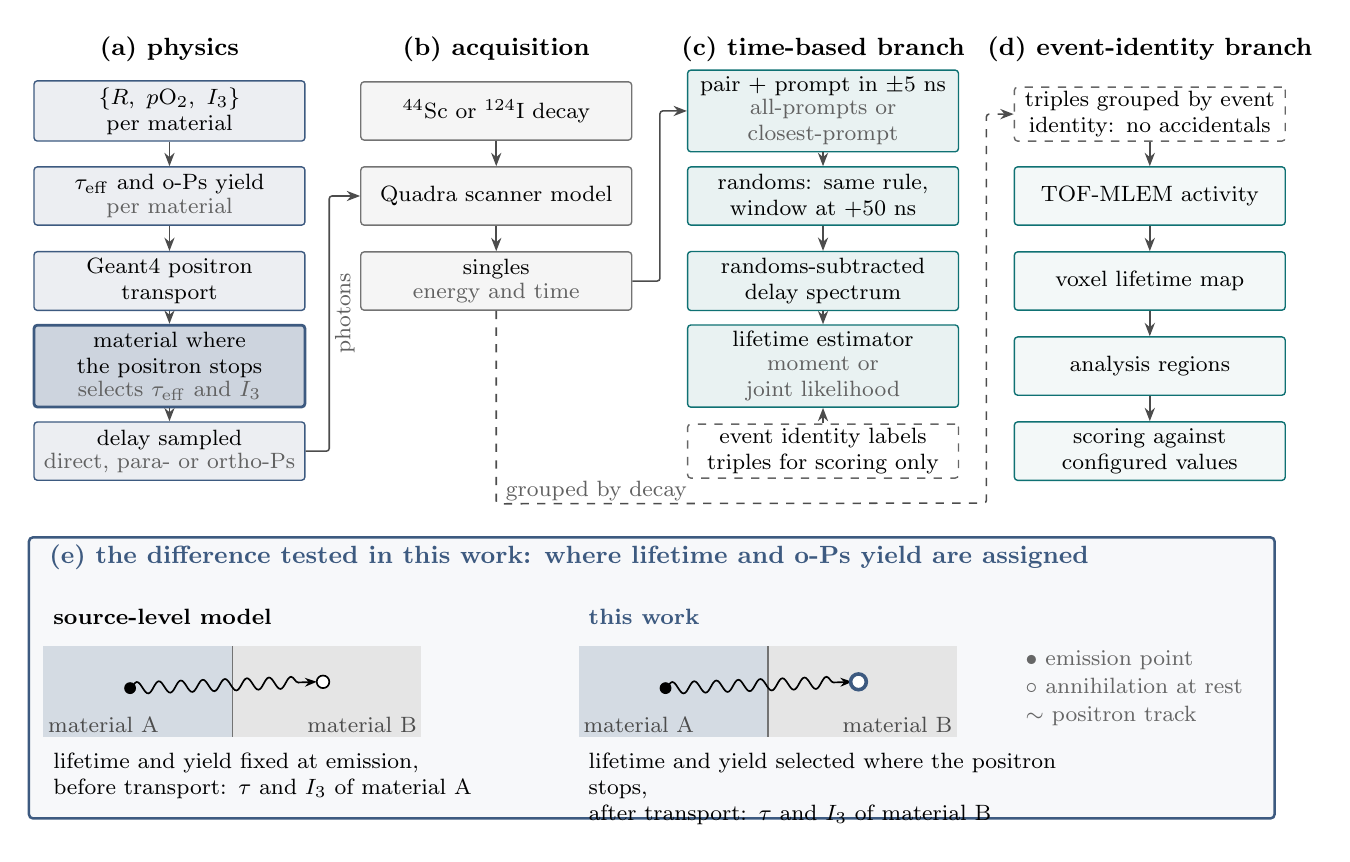
\begin{tikzpicture}[x=1cm, y=1cm]
\def\dy{1.08}
% ---------------- (a) physics ----------------
\node[head] at (0, 0.5) {(a) physics};
\node[phy] (a1) at (0, 0)        {$\{R,\ p\mathrm{O}_2,\ I_3\}$ per material};
\node[phy] (a2) at (0, -\dy)     {$\tau_{\mathrm{eff}}$ and o-Ps yield\sd{per material}};
\node[phy] (a3) at (0, -2*\dy)   {Geant4 positron transport};
\node[key] (a4) at (0, -3*\dy)   {material where the positron stops\sd{selects $\tau_{\mathrm{eff}}$ and $I_3$}};
\node[phy] (a5) at (0, -4*\dy)   {delay sampled\sd{direct, para- or ortho-Ps}};
\foreach \i/\j in {a1/a2, a2/a3, a3/a4, a4/a5} \draw[arr] (\i) -- (\j);

% ---------------- (b) acquisition ----------------
\def\xb{4.15}
\node[head] at (\xb, 0.5) {(b) acquisition};
\node[acq] (b1) at (\xb, 0)        {$^{44}$Sc or $^{124}$I decay};
\node[acq] (b2) at (\xb, -\dy)     {Quadra scanner model};
\node[acq] (b3) at (\xb, -2*\dy)   {singles\sd{energy and time}};
\foreach \i/\j in {b1/b2, b2/b3} \draw[arr] (\i) -- (\j);

% ---------------- (c) time-based branch ----------------
\def\xc{8.3}
\node[head] at (\xc, 0.5) {(c) time-based branch};
\node[ana] (c1) at (\xc, 0)        {pair $+$ prompt in $\pm$5 ns\sd{all-prompts or closest-prompt}};
\node[ana] (c2) at (\xc, -\dy)     {randoms: same rule,\\ window at $+$50 ns};
\node[ana] (c3) at (\xc, -2*\dy)   {randoms-subtracted\\ delay spectrum};
\node[ana] (c4) at (\xc, -3*\dy)   {lifetime estimator\sd{moment or joint likelihood}};
\node[tag] (c5) at (\xc, -4*\dy)   {event identity labels\\ triples for scoring only};
\foreach \i/\j in {c1/c2, c2/c3, c3/c4} \draw[arr] (\i) -- (\j);
\draw[arr, dashed] (c5) -- (c4);

% ---------------- (d) event-identity branch ----------------
\def\xd{12.45}
\node[head] at (\xd, 0.5) {(d) event-identity branch};
\node[tag] (d0) at (\xd, -0.04)    {triples grouped by event\\identity: no accidentals};
\node[acq, draw=hgreen, fill=hgreen!5] (d1) at (\xd, -\dy)     {TOF-MLEM activity};
\node[acq, draw=hgreen, fill=hgreen!5] (d2) at (\xd, -2*\dy)   {voxel lifetime map};
\node[acq, draw=hgreen, fill=hgreen!5] (d3) at (\xd, -3*\dy)   {analysis regions};
\node[acq, draw=hgreen, fill=hgreen!5] (d4) at (\xd, -4*\dy)   {scoring against\\ configured values};
\foreach \i/\j in {d0/d1, d1/d2, d2/d3, d3/d4} \draw[arr] (\i) -- (\j);

% ---------------- cross links ----------------
\draw[arr] (a5.east) -- ++(0.3,0) |- (b2.west);
\node[sub, anchor=north, rotate=90, inner sep=1pt] at ($(a5.east)+(0.33,1.75)$) {photons};
\draw[arr] (b3.east) -- ++(0.35,0) |- (c1.west);
\draw[arr, dashed] (b3.south) -- ++(0,-2.45) -- ($(\xc/2+\xd/2, -2*\dy-0.37-2.45)$) |- (d0.west);
\node[sub, anchor=south west, inner sep=1pt] at ($(b3.south)+(0.08,-2.45)$) {grouped by decay};

% ---------------- lower panel: source-level versus stopping-point assignment ----------------
\def\yl{-7.95}
\newcommand{\geom}[1]{%
  \fill[hblue!22] (0,0) rectangle (2.4,1.15);
  \fill[black!10] (2.4,0) rectangle (4.8,1.15);
  \draw[black!55, line width=0.5pt] (2.4,0) -- (2.4,1.15);
  \node[font=\sev, text=black!70, anchor=south west, inner sep=1.5pt] at (0,0) {material A};
  \node[font=\sev, text=black!70, anchor=south east, inner sep=1.5pt] at (4.8,0) {material B};
  \fill[black] (1.1,0.62) circle (0.075);
  \draw[-{Stealth[length=1.5mm]}, line width=0.6pt, decorate,
        decoration={snake, amplitude=0.75mm, segment length=2.8mm, post length=1.5mm}] (1.1,0.62) -- (3.47,0.7);
  #1}
\begin{scope}[shift={(-1.6,\yl)}]
  \node[font=\fontsize{8.4}{9.4}\selectfont\bfseries, anchor=west] at (0, 1.52) {source-level model};
  \geom{\fill[white, draw=black, line width=0.6pt] (3.55,0.7) circle (0.08);}
  \node[anchor=north west, align=left, text width=62mm] at (0,-0.08) {lifetime and yield fixed at emission,\\ before transport: $\tau$ and $I_3$ of material A};
\end{scope}
\begin{scope}[shift={(5.2,\yl)}]
  \node[font=\fontsize{8.4}{9.4}\selectfont\bfseries, anchor=west, text=hblue] at (0, 1.52) {this work};
  \geom{\fill[white, draw=hblue, line width=1.3pt] (3.55,0.7) circle (0.10);}
  \node[anchor=north west, align=left, text width=62mm] at (0,-0.08) {lifetime and yield selected where the positron stops,\\ after transport: $\tau$ and $I_3$ of material B};
\end{scope}
\node[font=\sev, text=black!60, anchor=west, align=left] at (10.75, \yl+0.62) {$\bullet$ emission point\\[1pt]$\circ$ annihilation at rest\\[1pt]$\sim$ positron track};
\node[head, anchor=south west, text=hblue] at (-1.65, \yl+2.0) {(e) the difference tested in this work: where lifetime and o-Ps yield are assigned};
\begin{scope}[on background layer]
  \node[draw=hblue, fill=hblue!4, rounded corners=1.5pt, line width=0.9pt, fit={(-1.75,\yl-1.0) (14.0,\yl+2.5)}, inner sep=1pt] {};
\end{scope}
\end{tikzpicture}
\end{document}
